\section{Постановка задач}
Провести SP-расчет методом HF/6-31G-CIS. Привести следующие результаты:
\begin{itemize}
    \item[-] число заполненных МО, число заполненных и вакантных $\pi$-орбиталей, их номера;
    \item[-] определить наличие $n$-орбиталей;
    \item[-] сопоставить $\pi$- и $n$-орбитали с $\pi$- и $n$-орбиталями, получеными в работе №8;
    \item[-] для каждого рассчитанного возбужденного состояния определить тип состояния, энергию, конфигурационный состав;
    \item[-] определить, какому состоянию из числа полученных в работе №8 соответствует данное состояние;
    \item[-] степень согласия энергии возбуждений с энергиями соответствующих состояний, полученных в работе №8.  
\end{itemize}

\begin{figure}[H]
\centering
\captionsetup{justification=centering}
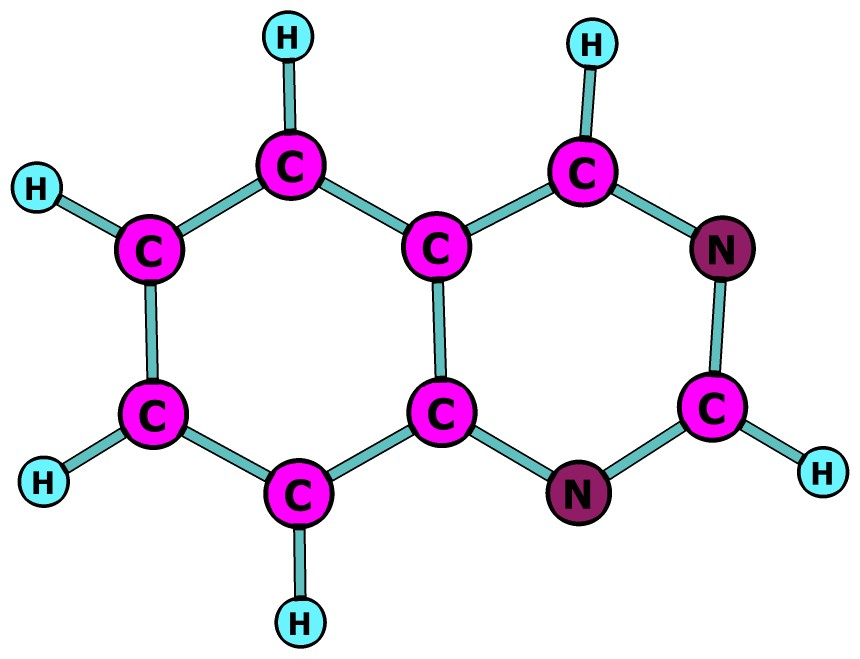
\includegraphics[scale=0.4]{fig/1.jpg}
\caption{Молекулы хиназолина}
\end{figure}